\documentclass[12pt]{article}

\usepackage[utf8]{inputenc}
\usepackage{latexsym,amsfonts,amssymb,amsthm,amsmath,graphicx}
\usepackage{hyperref}

\setlength{\parindent}{0in}
\setlength{\oddsidemargin}{0in}
\setlength{\textwidth}{6.5in}
\setlength{\textheight}{8.8in}
\setlength{\topmargin}{0in}
\setlength{\headheight}{18pt}

\newcommand{\Lc}{$\mathcal{L}$}


\title{ASTR 206 Lecture Notes}
\author{Simeon Bird}
% \date{October 14, 2019}

\begin{document}

\maketitle

\section{N-body effects: Evaporation and Ejection}
\subsection{The Relaxation Timescale}
\begin{figure}
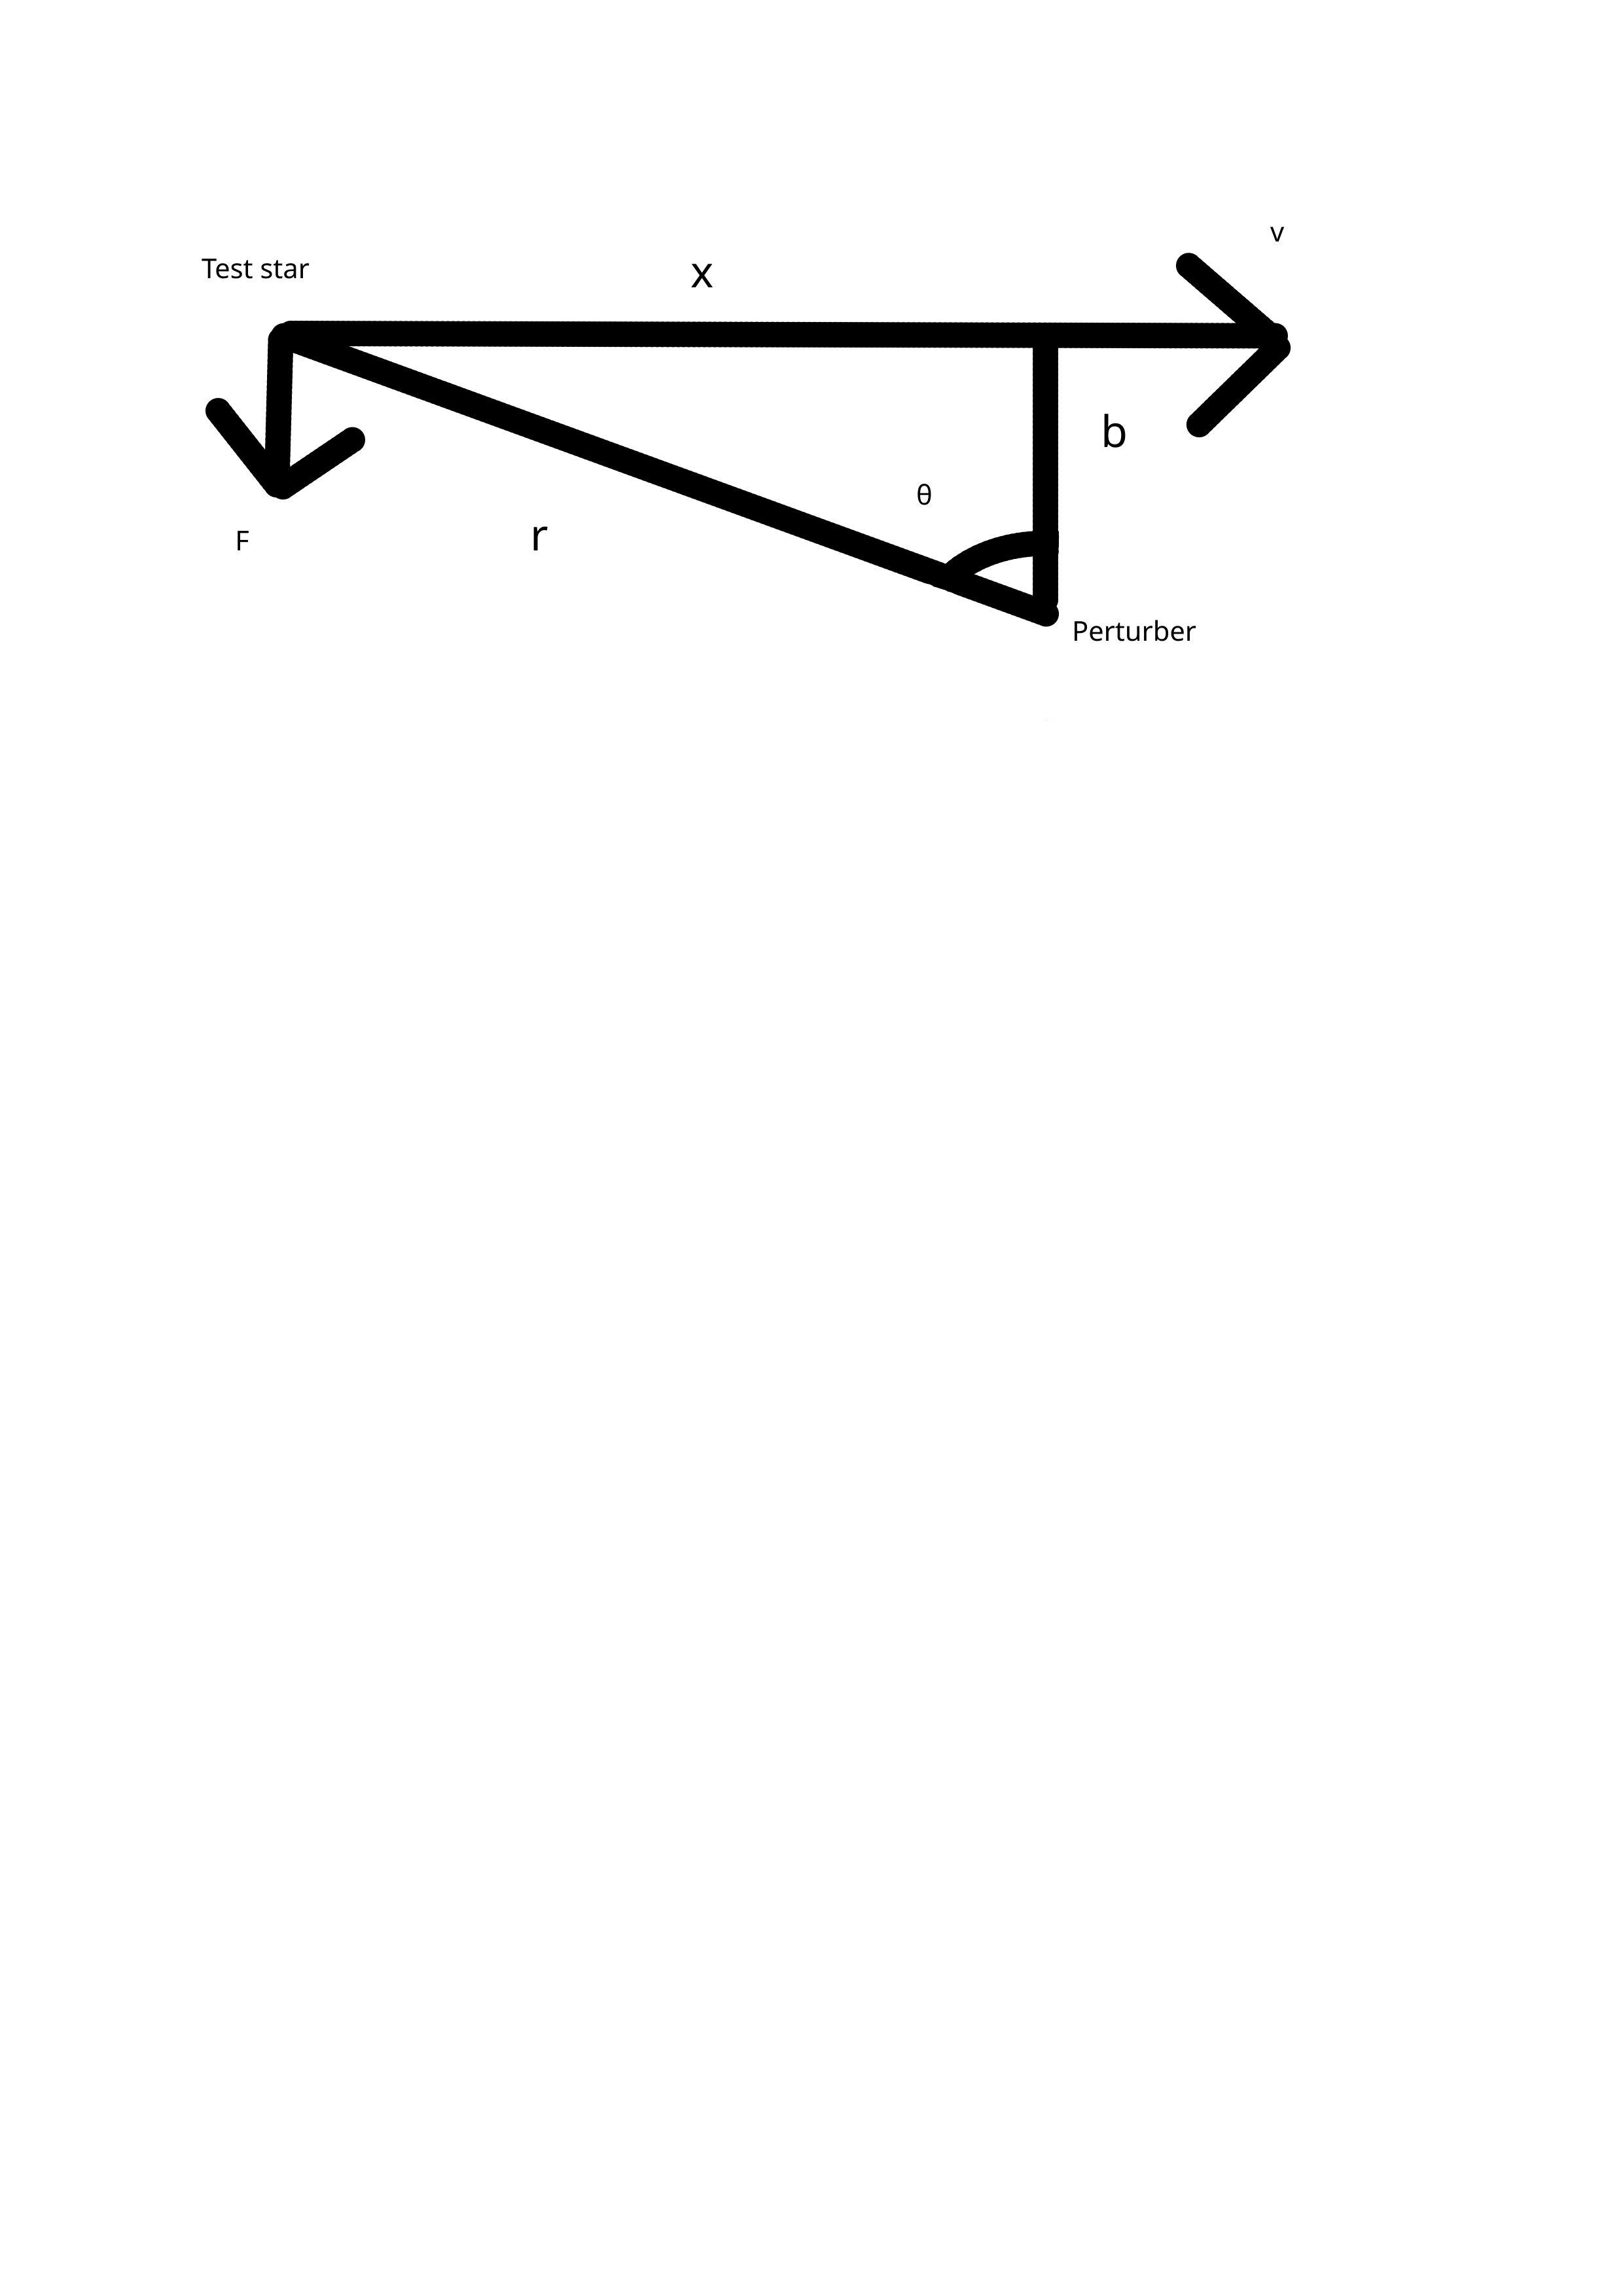
\includegraphics[trim={1cm 20cm 0.5cm 2.5cm},clip,scale=0.7]{BH_perturber.png}
\centering
\caption{Diagram of a close passage. A test star passes nearby a perturber, moving with velocity $v$. The impact parameter is $b$ and the distance is $x$. The perpendicular force from the perturber is $F$.}
\label{fig:close}
\end{figure}

This section is about N-Body specific effects, places where the discrete elements of the body matters. The section is based on Binney and Tremaine (second edition) Chapter 7.1 and 7.5. The derivation presented is the more approximate one in Binney and Tremaine. There is a more rigorous treatment based on the Fokker-Planck equation, but this treatment is more pedagogical.

For this section, let us imagine that a galaxy has N stars of identical mass m.

We want to know how encounters perturb a test star passing through, compared to a test star going through a smoothed potential. We will assume that in the absence of perturbations, objects are on virialised orbits in an underlying locally static potential. The goal is to find a characteristic timescale for these effects.


Figure~\ref{fig:close} shows an example perturbation, where a test star passes close to a perturber. We approximate stars as distant compared to their radii, so that other stars are off the ends of the diagram. The force on the test star is:
\begin{align}
 F &= \frac{G m^2}{b^2 + x^2} \cos \theta = \frac{G m^2 b}{(b^2 + x^2)^{3/2}} \\
 &\approx \frac{Gm^2}{b} \left( 1 + \left(\frac{v t}{b}\right)^2\right)^{-3/2} = m \dot{v}
\end{align}
So we can estimate a change in $v$, $\delta v$, as (defining $s = v t / b$):

\begin{align}
\delta v = \frac{G m}{b^2} \int^\infty_{-\infty} \frac{b}{v} (1 + s^2)^{-3/2} ds = 2\frac{G m}{b v}
\end{align}
The integration limits are infinity, as we are approximating the other stars as being much further away than $b$.

We also need to work out how many such encounters a random perturber will feel. We can assume that stars are randomly distributed with a uniform density. Since the galaxy has radius $R$, we define $\rho = N / (\pi R^2)$. So the average number of encounters at impact parameter $b$ is:
\begin{align}
 dn = \rho dV = N / (\pi R^2) 2 \pi b db = \frac{2 N}{R^2} b db
\end{align}
Notice that the sign of $dv$ is not set: it can be positive or negative and so by symmetry the average velocity perturbation is zero. However, the variance increases, expanding the galaxy over time.
\begin{align}
 |d v |^2 = \left(\frac{2 G m}{b v}\right)^2 dn \approx \left(\frac{2 G m}{b v}\right)^2 \frac{2 N}{R^2} b db
\end{align}
We want to integrate out $db$, but the lower integration limit has an infinite $dv$. However, this is because these orbits are not perturbations, but the formation of a binary. We can disallow them. Notice though that close not-quite-binary passages will lead to large $\delta v$. Our lower limit for a binary is: $b > b_{min} = G m / v^2$. The upper limit is $R$, the radius of the galaxy.
\begin{align}
 |\Delta v |^2 = \int^R_{b_{min}} |dv|^2 \approx 8 N \left(\frac{G m}{R v}\right)^2 \ln (R/b_{min})
\end{align}
and $v$ is the virial velocity $v^2 = G N m / R$. We next eliminate $R$ in favour of the virial velocity\footnote{Arguably since angular momentum is the conserved quantity, the virial velocity is the most useful physical quantity for assessing a galactic halo, rather than mass or radius. However, mass and radius are easier to measure.}. Also we have:
\begin{align}
\ln (R/b_{min}) \approx \frac{R v^2}{G m} \approx N
\end{align}
so that:
\begin{align}
 \left|\frac{\Delta v}{v} \right|^2 = 8 \frac{\ln N }{N}
\end{align}
So the number of crossings required to change $v$ by O(1) is $n_{relax} = \left|v / \Delta v \right|^2  = N / 8 \ln N$.
We define a \textbf{relaxation time} $t_{relax} = n_{relax} \times t_{cross}$.

So our dynamical time scale for N-body scattering is, using the total mass $M = Nm$:
\begin{align}
t_{relax} = \frac{N}{8 \ln N} \frac{R}{v} = \frac{N}{8 \ln N} \frac{R^{3/2}}{(G M)^{1/2}}
\end{align}
The more rigorous estimate in Binney and Tremaine comes out as:
\begin{align}
t_{relax} =\frac{ 0.14 N}{\ln (0.4 N)} \frac{R^{3/2}}{(G M)^{1/2}}
\end{align}
which is almost the same.

\subsection{Evaporation and Ejection}
There are two perturbative processes which matter for removing objects from a halo. These are evaporation and ejection.

\textbf{Ejection} occurs when a single close encounter between two stars leaves one of the stars with a speed exceeding the escape velocity.

\textbf{Evaporation} occurs when the cumulative effect of many encounters gradually increase the velocity until the particles escape.

Ejection is generally much rarer than evaporation. To see why, imagine a characteristic impact parameter than causes ejection, $b_{ej}$ and a (larger) $b_{evap}$ which can contribute to evaporation. The number of encounters with this $b$ will be $n \sim 2N (b/R)^2$, and since we know that $\Delta v \sim 1/b$, the overall change in velocity from evaporating encounters is $\Delta v \sim 2N b_{evap}$ while the change from ejection is $\Delta v \sim 2N b_{ej}$, which is smaller.

Numerically, we find that the timescale for a cluster to completely evaporate is:
\begin{align}
 t_{evap} = 100 t_{relax}
\end{align}
The time for `all' particles to be ejected (or settle into binaries) is the longer:
\begin{align}
 t_{ej} = 1000 \ln(N) t_{relax}
\end{align}

Dominating evaporation encounters are particles on elliptical orbits, where the apocenter is near the virial radius. The orbiting star picks up angular momentum when it is near the (denser) center of the star cluster. At some point it picks up enough momentum that the apocenter is no longer bound and the particle escapes. The remaining particles are then slightly more tightly bound (because the evaporating object took angular momentum with it) and so encounters are more frequent and the next object evaporates faster.

Many real star clusters have evaporation times longer than the age of the Universe: this is necessary as they often contain very old stars.

For dark matter (rather than `true' N-body) simulations, we want to suppress these discreteness effects: we do this by setting the softening length so that the relaxation times are longer than the simulation.

\subsection{Mass Segregation}

Consider what happens in an interaction if the two particles have separate masses. You might expect that equipartition of kinetic energy would occur. If we imagine two mass populations, one with mass $m_1$ and the other with mass $m_2$, and $m_2 > m_1$, this will lead to the lighter population $m_1$ inhabiting a sphere outside the heavier $m_2$.

On what timescale does energy equipartition happen? Naturally, a multiple of the relaxation time, since the mechanism for it is the close 2-body encounters discussed above. The actual timescale is:
\begin{align}
 t_{seg} = \frac{m_1}{m_2} t_{relax}
\end{align}
as might be expected from replacing the velocity change $dv$ above with the momentum change $dp$, as momentum is conserved in a collision.

This argument is originally due to Spitzer, and the original article and more details can be found here \url{https://articles.adsabs.harvard.edu/pdf/1969ApJ...158L.139S}

\section{Initial Conditions}

The preceding discussion suggests some considerations for the initial conditions of our model star cluster. We want to pick a setup which minimises transients from the initial conditions, near a steady state. This suggests a model which is virialised and where the particles sample a smooth density potential with a well-defined virial velocity. A common choice because it is analytically convenient is the Plummer profile:
\begin{align}
 \rho (r) = \frac{3 N m}{4 \pi a^3} \left(1 + \frac{r^2}{a^2} \right)^{-5/2}
\end{align}
which has velocity dispersion
\begin{align}
 \sigma^2(r) = \frac{G N m}{6 (r^2 + a^2)^{1/2}}.
\end{align}
This profile looks somewhat like the density distribution of star clusters, but mostly it is numerically convenient. You can find the algorithm for producing it in the appendix to this paper: \url{https://articles.adsabs.harvard.edu/pdf/1974A\%26A....37..183A}

\section{The Barnes-Hut Tree}

\begin{figure}
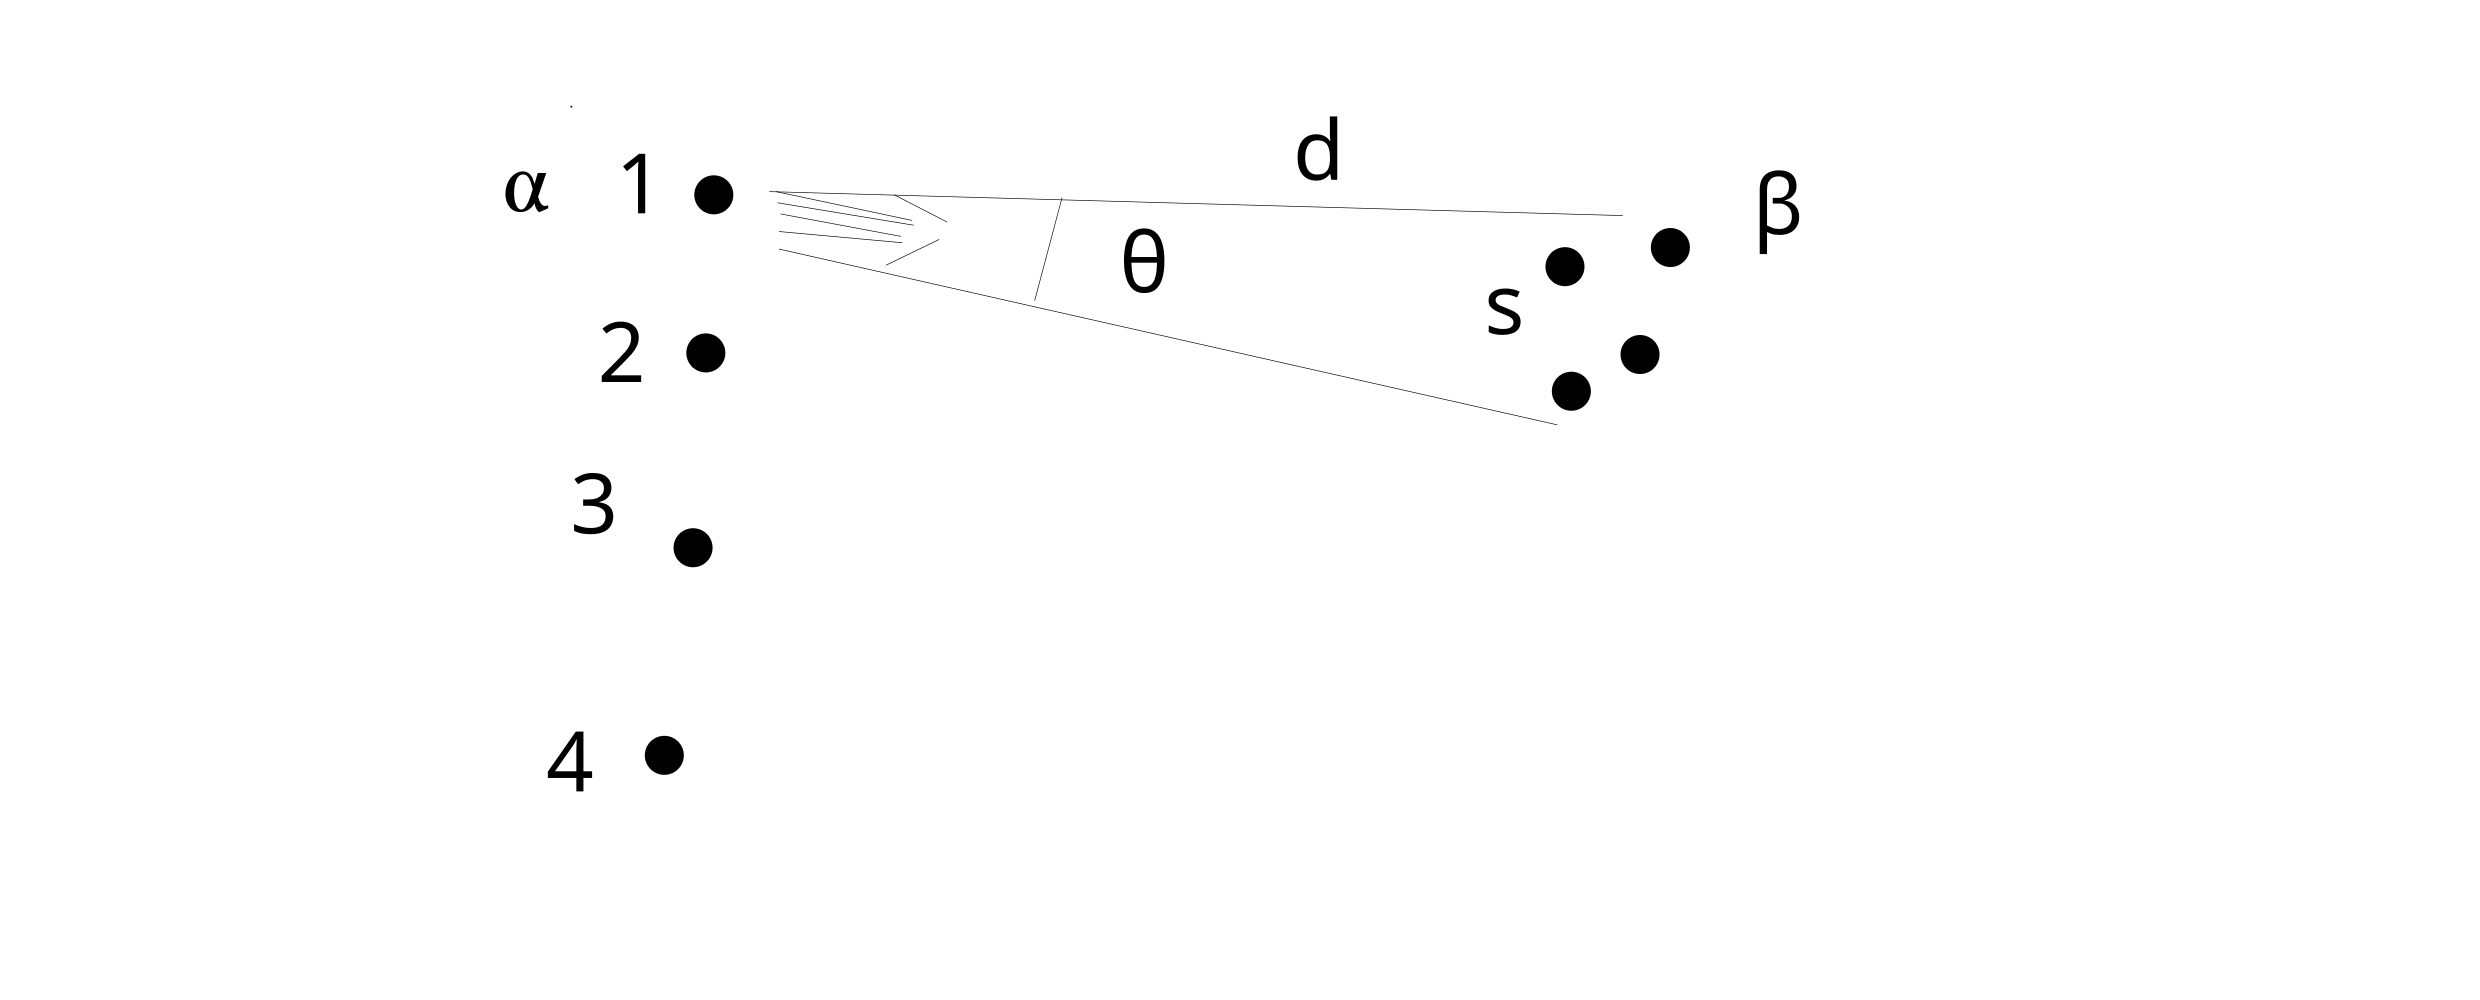
\includegraphics[scale=0.7]{bhtree.png}
\centering
\caption{For two groups of separated particles, the forces on $\alpha_{1,2,3,4}$ from $\beta_{1,2,3,4}$ are similar, and may be grouped.}
\label{fig:particles}
\end{figure}

Our code is still extremely slow! This is a problem. One easy way to make it faster by a factor of $2$ is to exploit the symmetry of Newton's laws: forces only need to be computed once for any pair.

In general, there are two techniques for finding faster algorithms. The first is to use divide-and-conquer: split the problem into two problems, each of half the size (this is how Fourier transforms are fast). The other is to identify calculations that duplicated and remove the duplication. Using the symmetry of Newton's laws is an example of the second.

The idea of the Barnes-Hut tree is that when you are far away from several objects, the gravitational force from those objects can be approximated as the force from a single object at the center of mass. For the objects in Figure~\ref{fig:particles}, we could write:

\begin{align}
 \Sigma_{i=1,4} (r_{\alpha_1} - r_{\beta_i})^{-2} \approx 4 (r_{\alpha_1} - \Sigma_i r_{\beta_i} / 4)^{-2}
\end{align}
This approximation is accurate only when the angular size of the far particles is small. Formally we could make an expansion in $\theta$. The condition used in the Barnes-Hut paper is:
\begin{align}
\theta \approx \frac{s}{d} < \theta_0 = 0.3
\end{align}
but different values of $\theta_0$ can be chosen depending your desired accuracy.

In practice we cover the space with a `tree', a hierarchical arrangement of regions. The base region covers the whole space, and each layer below subdivides it into $2^d$ sub-regions. The tree keeps being sub-divided until there are only a small number of particles in each small region. This means that there are more `layers' in the tree in denser regions. A more detailed description of the algorithm may be found here \url{http://arborjs.org/docs/barnes-hut}.

This model is O($N \log N$). To see why, think of a uniform distribution of particles. A constant angular size close by contains few particles, but at higher radii more and more are enclosed within each region.\footnote{You may ask: what if I arrange the particles so that larger radii contain fewer particles? Is a single force not then requiring N force evaluations? To which the answer is: for a particle in the center of the simulation, yes, but a particle on the edge may need only one evaluation. The average is $\log N$.} Evaluating the force for each particle requires moving only to $O(\log N)$ depth in the tree (notice that each tree layer contains half as many objects as the one above: this recursive halfing is key to the $\log N$ behaviour).

Gadget uses a different criterion, which behaves better in practice, although it is harder to justify analytically:
\begin{align}
 \frac{G N m}{d^2} \left(\frac{s}{d}\right)^2 \leq \alpha |a|
\end{align}
where $\alpha$ is an accuracy parameter around $2 \times 10^{-3}$ and $|a|$ is the acceleration at the last timestep. A geometric criterion is thus replaced with a dynamic one.

Tree structures are extremely useful in a variety of problems. Implementing this in python requires a tree node data structure containing a list of sub-nodes.

\section{Binary Detection}

We want to detect bound binaries in our code! How can we do that?

Let us first define what we mean by a bound binary: the normal condition is that the kinetic energy is insufficient to escape the gravitational potential. However, we are really interested in a slightly different problem: detection of binary black holes merging by gravitational radiation. The BH pair becomes gravitationally bound if the GW
emission exceeds the initial kinetic energy. The cross
section for this process is (See Quinlan et al 1989 or Mouri 2002):
\begin{eqnarray}
     \sigma^2 &=& \pi \left( \frac{85\, \pi}{3}
     \right)^{2/7} R_{s}^2 \left(\frac{v_\mathrm{bh}}{c}\right)^{-18/7}
\label{eqn:crosssection}
\end{eqnarray}
where $R_s$ is the Schwarzchild radius and $v_\mathrm{bh}$ is the relative velocity. Things become bound when their closest approach $b < \sigma$.

Notice that objects with very low relative velocities may have arbitrarily large $\sigma$. We do not want to detect these chance encounters as binaries, so we must also enforce a maximum separation. In addition, we should avoid 3-body effects, so we should ensure that only the two closest objects are allowed to merge.

We can implement this naively, or we can re-use our OctTree to do neighbour finding.

\end{document}
